\documentclass[aspectratio=169, table, 12pt]{beamer}

\usepackage{colortbl}
\usepackage{xcolor}
\usepackage{listings}
\usepackage{tabularx}
\usepackage{tikz}
\usetikzlibrary{arrows.meta, positioning, calc, fit, shapes.geometric}
\usepackage{pgfplots}
\pgfplotsset{compat=1.18}

\makeatletter
\def\input@path{{../theme/}}
\makeatother
\graphicspath{{../theme/}{../../figures/}}
\usetheme{Pradita}

\definecolor{praditagreen}{RGB}{37, 113, 71}

% Tema membuat garis tabel berwarna putih. Dikembalikan agar tabel terbaca.
\arrayrulecolor{black}
\setlength{\arrayrulewidth}{0.5pt}

% Kolom X rata kiri, dipakai pada tabel dengan kolom X yang sempit, agar
% spasi antarkata tidak meregang.
\newcolumntype{Y}{>{\raggedright\arraybackslash}X}

\lstdefinelanguage{bash}{
  keywords={},
  basicstyle=\ttfamily\scriptsize,
  ndkeywords={cd, curl, docker, echo, npx, python, python3, source},
  ndkeywordstyle=\color{purple}\bfseries,
  sensitive=true,
  commentstyle=\color{gray},
  numbers=none,
  breaklines=true,
  frame=lines,
  backgroundcolor=\color{lightgray!10},
  tabsize=2,
  comment=[l]{\#},
  showstringspaces=false
}

\lstdefinelanguage{TypeScript}{
  keywords={const, let, function, return, async, await, try, catch, throw,
            new, if, interface, void, export},
  ndkeywords={Promise, number, string, boolean, fetch, Error, Math, navigator,
              document, JSON},
  basicstyle=\ttfamily\scriptsize,
  keywordstyle=\color{blue}\bfseries,
  ndkeywordstyle=\color{purple}\bfseries,
  sensitive=true,
  commentstyle=\color{gray}\itshape,
  stringstyle=\color{red},
  numbers=none,
  breaklines=true,
  frame=lines,
  backgroundcolor=\color{lightgray!10},
  tabsize=2,
  comment=[l]{//},
  morestring=[b]",
  showstringspaces=false
}

% Gaya Python disamakan dengan naskah bab, tanpa nomor baris.
\lstdefinestyle{PythonStyle}{
  language=Python,
  basicstyle=\ttfamily\scriptsize,
  morekeywords={with, as, yield, async, await, match, case},
  keywordstyle=\color{blue}\bfseries,
  emph={psycopg, ConnectionPool, threading, defaultdict, partial},
  emphstyle=\color{purple}\bfseries,
  commentstyle=\color{gray}\itshape,
  stringstyle=\color{red},
  numbers=none,
  breaklines=true,
  frame=lines,
  backgroundcolor=\color{lightgray!10},
  tabsize=2,
  showstringspaces=false
}

% Berkas anggaran ditampilkan apa adanya, sehingga butuh gaya JSON sendiri.
\lstdefinelanguage{json}{
  basicstyle=\ttfamily\scriptsize,
  stringstyle=\color{red},
  commentstyle=\color{gray},
  numbers=none,
  breaklines=true,
  frame=lines,
  backgroundcolor=\color{lightgray!10},
  tabsize=2,
  showstringspaces=false,
  morestring=[b]"
}

\title{\Huge Performance\\ \vspace{10pt} Engineering}
\subtitle{IF140303 - Pengembangan Aplikasi Web}
\author{\textbf{Alfa Yohannis}}

\begin{document}

\frame{\titlepage}

\begin{frame}[fragile]
  \frametitle{Isi Pertemuan}
  \vspace{14pt}
  \begin{columns}[t]
    \column{0.5\textwidth}
    {\small\tableofcontents[sections={1-7}]}

    \column{0.5\textwidth}
    {\small\tableofcontents[sections={8-14}]}
  \end{columns}
\end{frame}

\begin{frame}{\hfill}
  \centering
  \Huge{\textbf{Kapan sebuah aplikasi\\dinyatakan cukup cepat?}}
\end{frame}

\section{Tujuan dan Kerangka Bahasan}

\begin{frame}{\hfill}
  \centering
  \Huge{\textbf{Tujuan dan Kerangka Bahasan}}
\end{frame}

\begin{frame}{{\Large Tujuan Pembelajaran}}
  \vspace{10pt}
  \begin{itemize}
    \item Menetapkan anggaran performa berupa angka, yaitu p95 tiap alamat,
          ukuran jawaban, dan ambang Core Web Vitals, lalu menegakkannya
          sebagai \textit{gate} otomatis.
    \item Mengukur aplikasi di bawah beban memakai \textit{load generator},
          lalu membaca titik jenuh dari hubungan antara konkurensi,
          \textit{throughput}, dan latensi.
    \item Menemukan bagian termahal lewat \textit{profiling}, lalu membedakan
          perbaikan yang menyentuh sebabnya dari perbaikan yang hanya
          menyentuh gejalanya.
  \end{itemize}
\end{frame}

\begin{frame}{{\Large Yang Belum Ada dari Tiga Bab Sebelumnya}}
  \vspace{10pt}
  \begin{itemize}
    \item Bab 2 menetapkan \textit{baseline} berupa angka.
    \item Bab 3 memperbaiki \textit{query} yang boros, Bab 4 menghapus perhitungan
          yang diulang-ulang.
    \item Yang belum ada: aturan yang menyatakan kapan aplikasi dinyatakan
          cukup cepat.
  \end{itemize}
  \vspace{8pt}
  {\footnotesize Tanpa aturan itu, perbaikan performa berhenti ketika
  seseorang merasa sudah cukup, bukan ketika angkanya tercapai.}
\end{frame}

\begin{frame}{{\Large Satu Putaran yang Berulang}}
  \vspace{16pt}
  \centering
  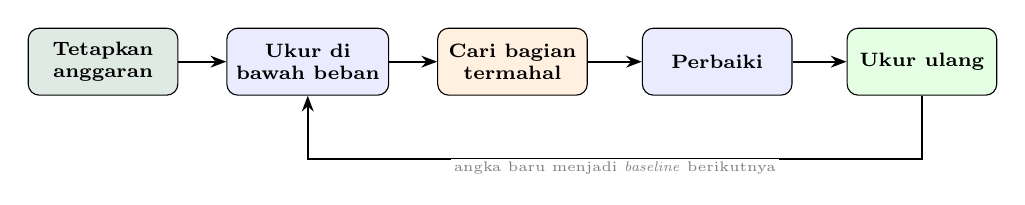
\begin{tikzpicture}[
    font=\scriptsize,
    kotak/.style={draw, rounded corners, minimum height=0.85cm,
                  minimum width=1.9cm, align=center, font=\scriptsize\bfseries},
    panah/.style={-{Stealth[length=2mm]}, thick}
  ]
    \node[kotak, fill=praditagreen!15] (anggar) at (0,0) {Tetapkan\\anggaran};
    \node[kotak, fill=blue!8] (ukur) at (2.6,0) {Ukur di\\bawah beban};
    \node[kotak, fill=orange!12] (profil) at (5.2,0) {Cari bagian\\termahal};
    \node[kotak, fill=blue!8] (perbaiki) at (7.8,0) {Perbaiki};
    \node[kotak, fill=green!10] (ulang) at (10.4,0) {Ukur ulang};

    \draw[panah] (anggar) -- (ukur);
    \draw[panah] (ukur) -- (profil);
    \draw[panah] (profil) -- (perbaiki);
    \draw[panah] (perbaiki) -- (ulang);
    \draw[panah] (ulang.south) -- ++(0,-0.8) -| (ukur.south);
    \node[font=\tiny, gray, anchor=north, fill=white, inner sep=1pt]
      at (6.5,-1.225) {angka baru menjadi \textit{baseline} berikutnya};
  \end{tikzpicture}

  \vspace{14pt}
  {\footnotesize Tiap langkah menghasilkan angka, dan angka itulah yang
  memutuskan langkah berikutnya.}
\end{frame}

\section{Anggaran Performa}

\begin{frame}{\hfill}
  \centering
  \Huge{\textbf{Anggaran Performa}}
\end{frame}

\begin{frame}{{\Large Tiga Jenis Batas}}
  \vspace{10pt}
  \begin{itemize}
    \item \textbf{Latensi} pada persentil tertentu, biasanya p95, karena
          rata-rata menyembunyikan pengalaman terburuk.
    \item \textbf{Ukuran jawaban} di kabel, karena byte yang dikirim
          menentukan waktu di jaringan yang lambat.
    \item \textbf{Core Web Vitals}, karena itulah yang benar-benar dirasakan
          pengguna di browser.
  \end{itemize}
  \vspace{8pt}
  {\footnotesize Ketiganya ditulis di satu berkas dan diperlakukan seperti
  kode: masuk repositori, ikut ditinjau, dan berubah lewat \textit{pull
  request}.}
\end{frame}

\begin{frame}{{\Large Analogi: Anggaran Belanja Kepanitiaan}}
  \vspace{14pt}
  \begin{itemize}
    \item Angkanya ditetapkan sebelum belanja dimulai, bukan sesudah nota
          menumpuk.
    \item Setiap pengeluaran baru harus muat di dalam pagu.
    \item Bila tidak muat, ada pengeluaran lain yang harus dipangkas.
  \end{itemize}
  \vspace{10pt}
  {\footnotesize Fitur baru boleh menambah waktu, asalkan masih muat, atau
  ada bagian lain yang dipercepat lebih dahulu.}
\end{frame}

\begin{frame}{{\Large Anggaran Bab Ini}}
  \vspace{6pt}
  \centering
  {\footnotesize
  \begin{tabularx}{\textwidth}{lYrr}
    \hline
    \textbf{Alamat} & \textbf{Isinya} & \textbf{p95} & \textbf{Ukuran} \\
    \hline
    \texttt{/api/katalog} & Satu halaman katalog, 20 baris & 60 ms & 8 KB \\
    \hline
    \texttt{/api/terlaris} & Agregat buku terlaris 30 hari & 400 ms & 2 KB \\
    \hline
    \texttt{/api/katalog-penuh} & Seluruh katalog, 50.000 baris & 60 ms & 8 KB \\
    \hline
    Core Web Vitals & LCP, INP, dan CLS pada persentil 75 &
      \multicolumn{2}{l}{2500 ms, 200 ms, 0,1} \\
    \hline
  \end{tabularx}}

  \vspace{8pt}
  {\footnotesize Dinilai pada 8 \textit{worker} dengan 25 permintaan tiap
  \textit{worker}.}
\end{frame}

\begin{frame}[fragile]{{\Large Anggaran sebagai Berkas}}
  \vspace{2pt}
\begin{lstlisting}[language=json, basicstyle=\ttfamily\tiny]
  "beban": {
    "jumlah_worker": 8,
    "permintaan_per_worker": 25
  },
  "alamat": [
    {
      "jalur": "/api/katalog?halaman=1&ukuran=20",
      "p95_ms": 60,
      "maks_kb": 8
    },

  "core_web_vitals": {
    "lcp_ms": 2500,
    "inp_ms": 200,
    "cls": 0.1
  }
\end{lstlisting}
  \vspace{2pt}
  {\footnotesize Dua bagian dari \texttt{anggaran.json}, dan dua alamat
  lainnya ditulis dengan pola yang sama. Alamat terberat ditaruh terakhir,
  agar pengukurannya tidak mencemari alamat sesudahnya.}
\end{frame}

\begin{frame}{{\Large Angka Lab dan Angka Lapangan Sering Tertukar}}
  \vspace{10pt}
  \begin{itemize}
    \item \textbf{Angka lab} diukur di komputer sendiri dengan beban buatan.
          Dapat diulang, sehingga layak dipakai sebagai \textit{gate} sebelum kode
          digabungkan.
    \item \textbf{Angka lapangan} dikumpulkan dari kunjungan nyata, sehingga
          memuat perangkat dan jaringan pengguna yang sesungguhnya.
  \end{itemize}
  \vspace{8pt}
  {\footnotesize Core Web Vitals dinilai pada persentil 75 dari kunjungan
  nyata. Karena itu pengumpulnya berupa JavaScript di halaman, bukan alat
  ukur di sisi server.}
\end{frame}

\begin{frame}{{\Large Tempat Anggaran Bekerja}}
  \vspace{16pt}
  \centering
  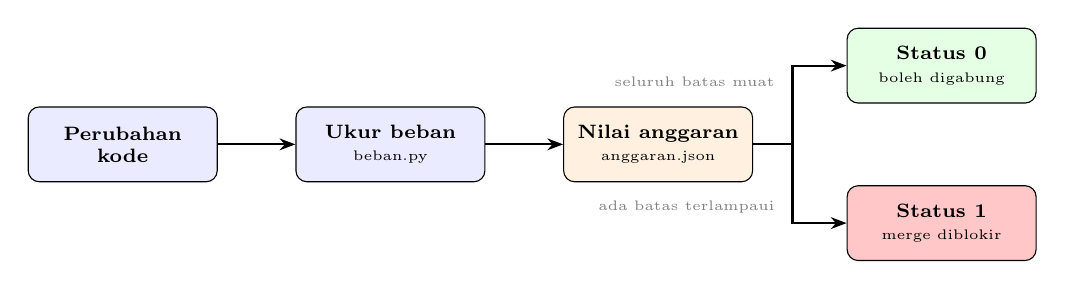
\begin{tikzpicture}[
    font=\scriptsize,
    kotak/.style={draw, rounded corners, minimum height=0.95cm,
                  minimum width=2.4cm, align=center, font=\scriptsize\bfseries},
    panah/.style={-{Stealth[length=2mm]}, thick}
  ]
    \node[kotak, fill=blue!8] (ubah) at (0,0) {Perubahan\\kode};
    \node[kotak, fill=blue!8] (ukur) at (3.4,0) {Ukur beban\\{\tiny\mdseries beban.py}};
    \node[kotak, fill=orange!12] (nilai) at (6.8,0) {Nilai anggaran\\{\tiny\mdseries anggaran.json}};
    \node[kotak, fill=green!10] (gabung) at (10.4,1.0) {Status 0\\{\tiny\mdseries boleh digabung}};
    \node[kotak, fill=red!22] (tolak) at (10.4,-1.0) {Status 1\\{\tiny\mdseries merge diblokir}};

    \draw[panah] (ubah) -- (ukur);
    \draw[panah] (ukur) -- (nilai);
    \draw[panah] (nilai.east) -- ++(0.5,0) |- (gabung.west);
    \draw[panah] (nilai.east) -- ++(0.5,0) |- (tolak.west);
    \node[font=\tiny, gray, anchor=east] at (8.4,0.8) {seluruh batas muat};
    \node[font=\tiny, gray, anchor=east] at (8.4,-0.8) {ada batas terlampaui};
  \end{tikzpicture}

  \vspace{12pt}
  {\footnotesize Vonisnya dibaca \textit{Continuous Integration} sebagai
  status keluar.}
\end{frame}

\begin{frame}[fragile]{{\Large Mengukur Core Web Vitals di Browser}}
  \vspace{2pt}
\begin{lstlisting}[language=TypeScript]
function catatLcp(daftar: PerformanceObserverEntryList): void {
  const entri = daftar.getEntries();
  const terakhir = entri[entri.length - 1];
  if (terakhir !== undefined) {
    laporan.lcp_ms = Math.round(terakhir.startTime);
  }
}

function kirimLaporan(): void {
  if (sudahDikirim) {
    return;
  }
  sudahDikirim = true;
  navigator.sendBeacon(ALAMAT_LAPORAN, JSON.stringify(laporan));
}
\end{lstlisting}
\end{frame}

\begin{frame}{{\Large Mengapa Dikirim Saat Halaman Ditinggalkan}}
  \vspace{14pt}
  \begin{itemize}
    \item INP baru diketahui setelah pengguna sempat berinteraksi.
    \item CLS masih dapat bertambah sampai halaman ditutup.
    \item \texttt{navigator.sendBeacon} membuat permintaannya tetap terkirim
          walaupun tabnya sudah ditutup.
  \end{itemize}
  \vspace{10pt}
  {\footnotesize Laporan yang dikirim saat halaman selesai dimuat akan selalu
  mencatat INP nol dan CLS yang belum lengkap.}
\end{frame}

\section{Metodologi Profiling}

\begin{frame}{\hfill}
  \centering
  \Huge{\textbf{Metodologi Profiling}}
\end{frame}

\begin{frame}{{\Large Dua Aturan Profiling}}
  \vspace{14pt}
  \begin{itemize}
    \item \textbf{Ukur lebih dahulu, baru perbaiki.} Tanpa itu, yang
          diperbaiki adalah bagian yang paling mudah ditebak, bukan bagian
          yang paling mahal.
    \item \textbf{Ukur pada tempat yang tepat.} Angka yang dirasakan klien
          dan angka yang terlihat di dalam server dapat berbeda jauh.
  \end{itemize}
  \vspace{10pt}
  {\footnotesize Selisih antara keduanya justru sering menjadi petunjuk
  terpenting, dan bab ini memuat satu contohnya.}
\end{frame}

\begin{frame}[fragile]{{\Large Memprofil di Dalam Proses}}
  \vspace{2pt}
\begin{lstlisting}[style=PythonStyle]
def kerjakan_katalog_penuh(pool_koneksi):
  """Mengerjakan seluruh pekerjaan alamat katalog penuh, sampai byte JSON."""
  return json.dumps(ambil_katalog_penuh(pool_koneksi)).encode()


def ulangi_pekerjaan(pekerjaan, pool_koneksi, jumlah_ulangan):
  """Menjalankan satu pekerjaan berulang kali, lalu melaporkan ukuran akhirnya.

  Diulang agar waktu tiap fungsi terkumpul cukup banyak untuk dibandingkan,
  bukan tenggelam oleh derajat ketelitian pengukur waktunya.
  """
  isi_jawaban = b""
  for _ in range(jumlah_ulangan):
    isi_jawaban = pekerjaan(pool_koneksi)
  return isi_jawaban
\end{lstlisting}
  \vspace{2pt}
  {\footnotesize Memakai \texttt{cProfile} dari pustaka standar Python, tanpa
  melewati jaringan.}
\end{frame}

\begin{frame}{{\Large Fungsi Termahal: Katalog Penuh}}
  \vspace{6pt}
  \centering
  {\footnotesize
  \begin{tabularx}{\textwidth}{Yrr}
    \hline
    \textbf{Fungsi} & \textbf{Kumulatif} & \textbf{Bagian} \\
    \hline
    Seluruh pekerjaan satu alamat & 7,52 s & 100\% \\
    \hline
    \texttt{ambil\_katalog\_penuh}, \textit{query} dan pembentukan kamus & 5,10 s & 68\% \\
    \hline
    \texttt{json.dumps}, serialisasi jawaban & 1,99 s & 26\% \\
    \hline
    \texttt{baris\_menjadi\_kamus}, dipanggil 1.000.000 kali & 1,61 s & 21\% \\
    \hline
    \texttt{fetchall}, memindahkan baris ke memori & 1,28 s & 17\% \\
    \hline
  \end{tabularx}}

  \vspace{8pt}
  {\footnotesize 20 ulangan, diurutkan menurut waktu kumulatif.}
\end{frame}

\begin{frame}{{\Large Dua Profil, Dua Kesimpulan}}
  \vspace{12pt}
  \begin{itemize}
    \item \textbf{Katalog penuh.} Waktu habis di memindahkan dan mengubah
          50.000 baris menjadi teks. \textit{Query} yang lebih pintar tidak menolong,
          karena yang mahal adalah jumlah barisnya.
    \item \textbf{Agregat.} Dari 3,89 detik untuk 20 ulangan, 3,84 detik atau
          99 persen dihabiskan di \texttt{connection.wait}, yaitu menunggu
          basis data.
  \end{itemize}
  \vspace{8pt}
  {\footnotesize Perbaikan katalog penuh: kirim lebih sedikit baris.
  Perbaikan agregat: perbaiki \textit{query}-nya seperti Bab 3, atau simpan hasilnya
  seperti Bab 4. Tidak ada yang dapat diperbaiki di kode aplikasinya.}
\end{frame}

\begin{frame}{{\Large Ketika Klien dan Server Tidak Sepakat}}
  \vspace{12pt}
  \begin{itemize}
    \item Profil sisi server alamat katalog berhalaman: di bawah satu
          milidetik.
    \item \textit{Load generator} mencatat 43,06 milidetik pada satu
          \textit{worker}.
    \item Selisih sebesar itu tidak mungkin berasal dari kode yang sudah
          diprofil.
  \end{itemize}
  \vspace{10pt}
  {\footnotesize Penyebabnya ada di lapisan transport, bukan di aplikasi.}
\end{frame}

\begin{frame}{{\Large Nagle Bertemu Delayed ACK}}
  \vspace{12pt}
  \begin{itemize}
    \item Header dan isi jawaban ditulis sebagai dua segmen TCP yang terpisah.
    \item Algoritma Nagle menahan segmen kecil kedua sampai segmen pertama
          menerima ACK (\textit{acknowledge}), yaitu tanda terima dari
          penerima.
    \item Penerima justru menunda ACK-nya.
    \item Keduanya bertemu pada tambahan tetap sekitar 40 milidetik untuk tiap
          jawaban kecil.
  \end{itemize}
  \vspace{8pt}
  {\footnotesize Obatnya satu baris: \texttt{disable\_nagle\_algorithm = True}
  pada penangan permintaan, yang menyalakan \texttt{TCP\_NODELAY}.}
\end{frame}

\begin{frame}{{\Large Sebelum dan Sesudah TCP\_NODELAY}}
  \vspace{6pt}
  \centering
  {\footnotesize
  \begin{tabularx}{\textwidth}{Yrrr}
    \hline
    \textbf{Alamat dan beban} & \textbf{Sebelum} & \textbf{Sesudah} & \textbf{Rasio} \\
    \hline
    \texttt{/api/katalog}, 1 \textit{worker} & 43,06 & 0,58 & 74$\times$ \\
    \hline
    \texttt{/api/katalog}, 8 \textit{worker} & 42,99 & 2,90 & 15$\times$ \\
    \hline
    \texttt{/api/terlaris}, 1 \textit{worker} & 125,44 & 76,53 & 1,6$\times$ \\
    \hline
    \texttt{/api/katalog-penuh}, 1 \textit{worker} & 149,48 & 157,83 & 0,9$\times$ \\
    \hline
  \end{tabularx}}

  \vspace{8pt}
  {\footnotesize p50 dalam milidetik. Baris terakhir sengaja dibiarkan apa
  adanya: jawaban katalog penuh besar, sehingga segmennya tidak pernah kecil
  dan tambahan 40 milidetik itu tidak pernah muncul.}
\end{frame}

\section{Ukuran Jawaban dan Analisis Bundle}

\begin{frame}{\hfill}
  \centering
  \Huge{\textbf{Ukuran Jawaban\\dan Analisis Bundle}}
\end{frame}

\begin{frame}{{\Large Byte Ikut Dianggarkan}}
  \vspace{14pt}
  \begin{itemize}
    \item Waktu yang dirasakan pengguna ditentukan kecepatan server dan
          banyaknya byte yang melintas.
    \item Pada jaringan 4G yang lambat, satu megabyte tambahan berarti detik
          tambahan, berapa pun cepatnya basis data.
  \end{itemize}
  \vspace{10pt}
  {\footnotesize Karena itu anggaran memuat batas ukuran, bukan hanya batas
  waktu.}
\end{frame}

\begin{frame}{{\Large Ukuran Jawaban di Kabel}}
  \vspace{6pt}
  \centering
  {\footnotesize
  \begin{tabularx}{\textwidth}{Yrrr}
    \hline
    \textbf{Alamat} & \textbf{Tanpa gzip} & \textbf{Dengan gzip} & \textbf{Rasio} \\
    \hline
    \texttt{/api/katalog}, 20 baris & 1.545 B & 292 B & 5,3$\times$ \\
    \hline
    \texttt{/api/terlaris}, 10 baris & 557 B & 557 B & 1,0$\times$ \\
    \hline
    \texttt{/api/katalog-penuh}, 50.000 baris & 4.214.788 B & 281.905 B & 15,0$\times$ \\
    \hline
  \end{tabularx}}

  \vspace{8pt}
  {\footnotesize Diukur dengan \texttt{curl}, dengan dan tanpa
  \texttt{Accept-Encoding: gzip}. Baris tengah tidak berubah sama sekali.}
\end{frame}

\begin{frame}[fragile]{{\Large Jawaban Kecil Tidak Di-compress}}
  \vspace{2pt}
\begin{lstlisting}[style=PythonStyle]
def compress_bila_diminta(isi_jawaban, nilai_accept_encoding):
  """Meng-compress isi jawaban bila klien menerima gzip dan isinya cukup besar.

  Mengembalikan pasangan (isi, nilai Content-Encoding atau None). Jawaban
  kecil dibiarkan apa adanya, karena gzip justru menambah byte dan waktu.
  """
  menerima_gzip = "gzip" in (nilai_accept_encoding or "")
  if not menerima_gzip or len(isi_jawaban) < BATAS_COMPRESS_BYTE:
    return isi_jawaban, None
  return gzip.compress(isi_jawaban), "gzip"
\end{lstlisting}
  \vspace{2pt}
  {\footnotesize Batasnya 1.024 byte. Jawaban 557 byte itu lewat tanpa
  disentuh.}
\end{frame}

\begin{frame}{{\Large Compress Memperkecil Gejala}}
  \vspace{14pt}
  \begin{itemize}
    \item Rasio 15 kali lipat pada katalog penuh memang mengesankan.
    \item Namun 281.905 byte tetap 34 kali lipat lebih besar daripada
          anggaran 8 kibibyte.
    \item Sebabnya jumlah baris yang dikirim, bukan cara mengemasnya.
  \end{itemize}
  \vspace{10pt}
  {\footnotesize Perbaikan yang benar memotong jumlah barisnya, dan itulah
  yang dilakukan alamat katalog berhalaman.}
\end{frame}

\begin{frame}{{\Large Tiga Cara Menekan Ukuran Bundle}}
  \vspace{14pt}
  \begin{itemize}
    \item \textit{Tree shaking} membuang kode yang tidak pernah dipanggil saat
          \textit{bundle} disusun.
    \item \textit{Code splitting} memecah \textit{bundle} menurut halaman atau
          fitur, sehingga halaman katalog tidak ikut mengunduh kode halaman
          laporan.
    \item \textit{Lazy loading} menunda pengunduhan potongan itu sampai
          benar-benar dibutuhkan.
  \end{itemize}
  \vspace{8pt}
  {\footnotesize Tiap kilobyte JavaScript harus diunduh, di-\textit{parse},
  lalu dijalankan, dan ketiganya menunda interaksi pertama.}
\end{frame}

\begin{frame}{{\Large Ukuran Berkas Halaman Demo}}
  \vspace{6pt}
  \centering
  {\footnotesize
  \begin{tabularx}{\textwidth}{Yrr}
    \hline
    \textbf{Berkas} & \textbf{Apa adanya} & \textbf{Dengan gzip} \\
    \hline
    \texttt{statis/index.html} & 832 B & 482 B \\
    \hline
    \texttt{statis/web-vitals.js} & 2.615 B & 1.156 B \\
    \hline
    \texttt{statis/katalog.js} & 1.591 B & 817 B \\
    \hline
    Seluruh JavaScript halaman & 4.206 B & 1.697 B \\
    \hline
  \end{tabularx}}

  \vspace{8pt}
  {\footnotesize Angkanya kecil karena halamannya memang kecil. Yang dibawa
  bukan angkanya, melainkan kebiasaannya: ukuran diukur pada tiap perubahan,
  lalu dibandingkan dengan anggaran.}
\end{frame}

\section{Lazy Loading, Gambar, dan Font}

\begin{frame}{\hfill}
  \centering
  \Huge{\textbf{Lazy Loading, Gambar,\\dan Font}}
\end{frame}

\begin{frame}{{\Large Empat Perbaikan, dari yang Paling Murah}}
  \vspace{8pt}
  \begin{enumerate}
    \item Ukuran gambar disesuaikan dengan ukuran tampilnya. Gambar 2.000
          piksel yang ditampilkan selebar 400 piksel membuang sekitar 96
          persen pikselnya.
    \item Format modern dipakai, misalnya WebP atau AVIF, yang pada mutu
          setara menghasilkan berkas jauh lebih kecil daripada JPEG.
    \item Gambar di luar layar pertama ditunda dengan
          \texttt{loading="lazy"}, sehingga tidak ikut berebut pita dengan
          gambar yang menentukan LCP.
    \item Font diberi \texttt{font-display: swap}, dan hanya varian yang
          dipakai yang diunduh.
  \end{enumerate}
  \vspace{4pt}
  {\footnotesize Gambar adalah penyumbang byte terbesar pada halaman web
  kebanyakan, dan font menyusul di belakangnya.}
\end{frame}

\begin{frame}{{\Large Gambar LCP Justru Tidak Ditunda}}
  \vspace{14pt}
  \begin{itemize}
    \item Gambar yang menjadi elemen LCP tidak boleh diberi
          \texttt{loading="lazy"}.
    \item Penundaan itu memperlambat metrik yang sedang diperbaiki.
    \item Untuk gambar tersebut yang dipakai kebalikannya, yaitu
          \texttt{fetchpriority="high"}.
  \end{itemize}
  \vspace{10pt}
  {\footnotesize Satu atribut yang sama dapat memperbaiki atau merusak,
  bergantung pada elemen mana yang dikenainya.}
\end{frame}

\begin{frame}{{\Large Ukuran Gambar dan CLS}}
  \vspace{14pt}
  \begin{itemize}
    \item Elemen gambar tanpa \texttt{width} dan \texttt{height} membuat
          browser tidak dapat menyediakan ruangnya lebih dahulu.
    \item Teks di bawahnya melompat begitu gambarnya tiba.
    \item Pergeseran itu terbaca sebagai CLS oleh pengukur di halaman.
  \end{itemize}
  \vspace{10pt}
  {\footnotesize Cara mencegahnya cukup mencantumkan ukurannya, tanpa
  perubahan logika aplikasi sama sekali.}
\end{frame}

\section{Streaming Server-Side Rendering}

\begin{frame}{\hfill}
  \centering
  \Huge{\textbf{Streaming\\Server-Side Rendering}}
\end{frame}

\begin{frame}{{\Large Mengirim Bagian yang Sudah Siap}}
  \vspace{12pt}
  \begin{itemize}
    \item Halaman yang dirakit di server biasanya dikirim setelah seluruh
          datanya siap, sehingga pengguna menatap layar kosong.
    \item \textit{Streaming} mengubah urutannya: bagian yang siap dikirim
          lebih dahulu, sisanya menyusul dalam potongan berikutnya.
    \item Mekanismenya \textit{chunked transfer encoding} milik HTTP/1.1.
  \end{itemize}
  \vspace{8pt}
  {\footnotesize Analoginya seperti menyajikan makanan di kantin. Total waktu
  memasak sama, tetapi yang menunggu merasakan keduanya sangat berbeda.}
\end{frame}

\begin{frame}[fragile]{{\Large Header Dulu, Baru Menghitung}}
  \vspace{2pt}
\begin{lstlisting}[style=PythonStyle]
  def layani_terlaris_streaming(self):
    """Mengirim header lebih dahulu, baru menghitung agregatnya.

    Bagian yang sudah siap dikirim duluan, sehingga waktu sampai byte pertama
    tidak menunggu query selesai. Waktu total tidak berubah.
    """
    self.send_response(200)
    self.send_header("Content-Type", "application/json")
    self.send_header("Cache-Control", CACHE_CONTROL_API)
    self.send_header("Transfer-Encoding", "chunked")
    self.end_headers()
    self.kirim_potongan(b'{"item":[')
    daftar_terlaris = jalankan_query_terlaris(self.server.pool_koneksi)
\end{lstlisting}
\end{frame}

\begin{frame}{{\Large Waktu sampai Byte Pertama}}
  \vspace{6pt}
  \centering
  {\footnotesize
  \begin{tabularx}{\textwidth}{Yrr}
    \hline
    \textbf{Alamat} & \textbf{Byte pertama} & \textbf{Total} \\
    \hline
    \texttt{/api/terlaris} & 118 sampai 196 & 119 sampai 196 \\
    \hline
    \texttt{/api/terlaris-streaming} & 0,7 sampai 0,9 & 95 sampai 103 \\
    \hline
  \end{tabularx}}

  \vspace{8pt}
  {\footnotesize Dalam milidetik, tiga permintaan berurutan untuk tiap
  alamat, diukur dengan \texttt{curl}.}
\end{frame}

\begin{frame}{{\Large Memindahkan Waktu Tunggu, Bukan Menghapusnya}}
  \vspace{14pt}
  \begin{itemize}
    \item Waktu sampai byte pertama turun dari ratusan milidetik menjadi
          kurang dari satu milidetik.
    \item Waktu totalnya tidak membaik, dan memang tidak seharusnya membaik.
    \item Yang diperbaiki adalah pengalaman menunggu, sedangkan pekerjaannya
          tetap sama.
  \end{itemize}
  \vspace{10pt}
  {\footnotesize Perbaikan semacam ini tetap berharga, asalkan tidak
  dilaporkan sebagai penghematan waktu kerja.}
\end{frame}

\section{Tuning Basis Data dan Query}

\begin{frame}{\hfill}
  \centering
  \Huge{\textbf{Tuning Basis Data\\dan Query}}
\end{frame}

\begin{frame}{{\Large Berapa Baris yang Pantas Dikirim}}
  \vspace{14pt}
  \begin{itemize}
    \item Bab 3 menyetel \textit{query} lewat indeks.
    \item Bab 4 menghindari perhitungan berulang lewat \textit{cache}.
    \item Bab ini menambahkan penyetelan yang sering terlewat, yaitu jumlah
          baris dalam satu jawaban.
  \end{itemize}
  \vspace{10pt}
  {\footnotesize Dua alamat berikut menjawab kebutuhan yang sama, yaitu
  menampilkan katalog, dengan jumlah baris yang berbeda.}
\end{frame}

\begin{frame}{{\Large Berhalaman lawan Penuh}}
  \vspace{6pt}
  \centering
  {\footnotesize
  \begin{tabularx}{\textwidth}{Yrrr}
    \hline
    \textbf{Ukuran} & \textbf{Berhalaman} & \textbf{Penuh} & \textbf{Rasio} \\
    \hline
    p50 & 9,24 & 2.202,68 & 238$\times$ \\
    \hline
    p95 & 14,02 & 2.998,55 & 214$\times$ \\
    \hline
    \textit{Throughput}, permintaan per detik & 811,8 & 3,5 & 232$\times$ \\
    \hline
    Ukuran jawaban di kabel & 0,3 KB & 275,3 KB & 918$\times$ \\
    \hline
  \end{tabularx}}

  \vspace{8pt}
  {\footnotesize Waktu dalam milidetik, pada 8 \textit{worker}. Kedua alamat
  memakai tabel dan indeks yang sama. Yang berbeda hanya jumlah barisnya.}
\end{frame}

\begin{frame}[fragile]{{\Large Batas Halaman Ditegakkan di Server}}
  \vspace{2pt}
\begin{lstlisting}[style=PythonStyle]
def baca_parameter_halaman(query_alamat):
  """Membaca parameter halaman dan ukuran dari alamat, beserta batasnya.

  Ukuran dibatasi agar satu permintaan tidak dapat meminta seluruh tabel
  hanya dengan mengubah alamat.
  """
  parameter = parse_qs(query_alamat)
  halaman = max(1, int(parameter.get("halaman", ["1"])[0]))
  ukuran = int(parameter.get("ukuran", [str(UKURAN_HALAMAN_BAWAAN)])[0])
  return halaman, min(max(1, ukuran), UKURAN_HALAMAN_MAKSIMUM)
\end{lstlisting}
  \vspace{2pt}
  {\footnotesize Batas ukuran halaman ditentukan server, bukan dipercayakan
  kepada klien.}
\end{frame}

\begin{frame}{{\Large Dua Aturan dan Satu Perkecualian}}
  \vspace{12pt}
  \begin{itemize}
    \item Setiap alamat yang mengembalikan daftar wajib berhalaman.
    \item Kolom yang tidak dipakai tidak ikut diambil, karena tiap kolom
          menambah byte yang diubah dan dikirim.
    \item Alamat agregat menempuh jalan berbeda: barisnya hanya sepuluh,
          tetapi p95-nya 930,99 milidetik pada 8 \textit{worker}, jauh di
          atas anggaran 400 milidetik.
  \end{itemize}
  \vspace{8pt}
  {\footnotesize Profilnya menunjukkan 99 persen waktu dihabiskan menunggu
  basis data. Yang tersisa: simpan hasilnya seperti Bab 4, atau tambah
  kapasitas basis datanya.}
\end{frame}

\section{Load Testing dan Titik Jenuh}

\begin{frame}{\hfill}
  \centering
  \Huge{\textbf{Load Testing\\dan Titik Jenuh}}
\end{frame}

\begin{frame}{{\Large Mengukur Saat Sepi Menjawab Pertanyaan yang Salah}}
  \vspace{14pt}
  \begin{itemize}
    \item Pengguna datang bersamaan, dan perilaku sistem saat ramai tidak
          dapat ditebak dari perilakunya saat sepi.
    \item \textit{Load testing} memberi beban terkendali, lalu mencatat
          latensi dan \textit{throughput}-nya.
    \item Bentuk yang dipakai bab ini \textit{closed loop}: tiap
          \textit{worker} menunggu jawaban sebelum mengirim permintaan
          berikutnya.
  \end{itemize}
  \vspace{8pt}
  {\footnotesize Satu \textit{worker} berlaku seperti satu pengguna yang
  sabar, bukan seperti mesin yang membanjiri server.}
\end{frame}

\begin{frame}[fragile]{{\Large Satu Worker di Dalam Load Generator}}
  \vspace{2pt}
\begin{lstlisting}[style=PythonStyle]
def jalankan_satu_worker(jalur, jumlah_permintaan, catatan):
  """Mengirim permintaan berurutan lewat satu koneksi, lalu mencatat hasilnya.

  Koneksi dibuka sekali dan dipakai ulang, sehingga yang terukur adalah waktu
  server, bukan waktu membuka koneksi baru.
  """
  koneksi = HTTPConnection(HOST_BAWAAN, PORT_BAWAAN, timeout=BATAS_WAKTU_DETIK)
  header = {"Accept-Encoding": "gzip"}
  for _ in range(jumlah_permintaan):
    waktu_mulai = time.perf_counter()
\end{lstlisting}
\end{frame}

\begin{frame}{{\Large Menaikkan Konkurensi pada Alamat Agregat}}
  \vspace{4pt}
  \centering
  {\scriptsize
  \begin{tabularx}{\textwidth}{rrrrY}
    \hline
    \textbf{Worker} & \textbf{p50} & \textbf{p95} & \textbf{Per detik} & \textbf{Yang terjadi} \\
    \hline
    1 & 156,83 & 214,61 & 6,0 & Tidak ada antrean \\
    \hline
    2 & 172,61 & 184,05 & 11,6 & Kapasitas masih terpakai \\
    \hline
    4 & 302,01 & 409,19 & 12,2 & Mulai jenuh \\
    \hline
    8 & 514,98 & 835,65 & 13,6 & Tambahan beban menjadi antrean \\
    \hline
    16 & 1.210,84 & 2.153,35 & 11,6 & \textit{Throughput} turun \\
    \hline
    32 & 2.794,87 & 3.945,97 & 11,0 & Latensi meledak, hasil tetap \\
    \hline
  \end{tabularx}}

  \vspace{6pt}
  {\footnotesize Waktu dalam milidetik, 15 permintaan tiap \textit{worker}.}
\end{frame}

\begin{frame}{{\Large Titik Jenuh dalam Satu Gambar}}
  \vspace{4pt}
  \centering
  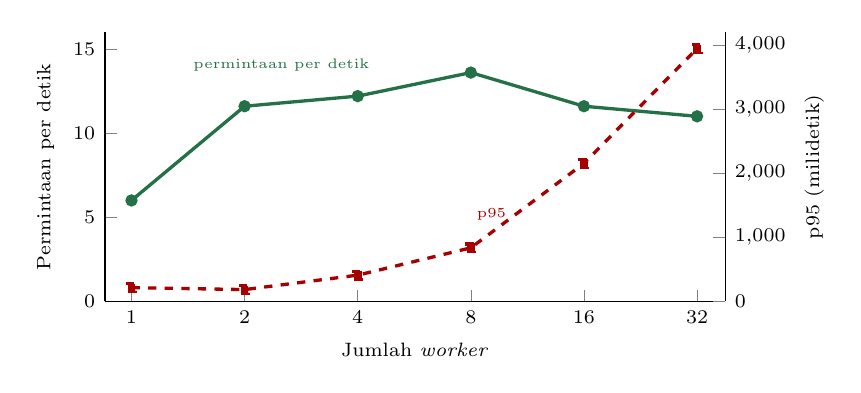
\begin{tikzpicture}[font=\scriptsize]
    \begin{axis}[
      width=0.78\textwidth, height=5.0cm,
      xmode=log, log basis x=2, xmin=0.85, xmax=38,
      xtick={1,2,4,8,16,32}, xticklabels={1,2,4,8,16,32},
      xlabel={Jumlah \textit{worker}}, ylabel={Permintaan per detik},
      ymin=0, ymax=16, axis y line*=left, axis x line*=bottom,
    ]
      \addplot[praditagreen, very thick, mark=*, mark size=1.6]
        coordinates {(1,6.0) (2,11.6) (4,12.2) (8,13.6) (16,11.6) (32,11.0)};
    \end{axis}
    \begin{axis}[
      width=0.78\textwidth, height=5.0cm,
      xmode=log, log basis x=2, xmin=0.85, xmax=38,
      axis y line*=right, axis x line=none, xtick=\empty,
      ylabel={p95 (milidetik)}, ymin=0, ymax=4200,
    ]
      \addplot[red!65!black, very thick, dashed, mark=square*, mark size=1.4]
        coordinates {(1,214.61) (2,184.05) (4,409.19) (8,835.65)
                     (16,2153.35) (32,3945.97)};
    \end{axis}
    \node[font=\tiny, praditagreen, anchor=west] at (1.0,3.0) {permintaan per detik};
    \node[font=\tiny, red!65!black, anchor=west] at (4.6,1.1) {p95};
  \end{tikzpicture}

  \vspace{4pt}
  {\footnotesize Sesudah titik jenuh, menambah \textit{worker} hanya
  menaikkan p95 tanpa menambah permintaan per detik.}
\end{frame}

\begin{frame}{{\Large Tiga Kesimpulan dari Titik Jenuh}}
  \vspace{14pt}
  \begin{itemize}
    \item Kapasitas sistem ini sekitar 13 permintaan per detik untuk alamat
          tersebut.
    \item Menambah \textit{worker} di atas titik jenuh tidak menambah
          kapasitas, hanya memindahkan waktu tunggu ke dalam antrean.
    \item Perbaikan yang benar menaikkan kapasitasnya, misalnya lewat
          \textit{cache} Bab 4, bukan menaikkan konkurensi.
  \end{itemize}
  \vspace{8pt}
  {\footnotesize Pada 32 \textit{worker}, p95 menjadi 18 kali lipat p95 pada
  satu \textit{worker}, sementara hasilnya justru sedikit lebih rendah.}
\end{frame}

\begin{frame}{{\Large Memeriksa Angka dengan Hukum Little}}
  \vspace{14pt}
  \begin{itemize}
    \item Jumlah permintaan yang sedang dikerjakan sama dengan
          \textit{throughput} dikalikan waktu tinggalnya.
    \item Pada baris 8 \textit{worker}: $13{,}6 \times 0{,}515 = 7{,}0$, dan
          angka itu memang mendekati 8.
  \end{itemize}
  \vspace{10pt}
  {\footnotesize Kecocokan tersebut menjadi pemeriksaan kewarasan. Bila
  ketiganya tidak konsisten, yang salah biasanya pengukurannya.}
\end{frame}

\begin{frame}{{\Large Menjaga Pengukuran Tetap Jujur}}
  \vspace{12pt}
  \begin{itemize}
    \item Alamat katalog penuh membaca seluruh tabel ratusan kali, sehingga
          halaman tabel lain terdorong keluar dari \textit{shared buffers}.
    \item Pengukuran alamat agregat tepat sesudahnya mencatat p95 sekitar
          1.000 milidetik, padahal dengan pemanasan 831 sampai 931 milidetik.
  \end{itemize}
  \vspace{8pt}
  Tiga aturan yang dipakai \textit{gate} anggaran:
  \begin{enumerate}
    \item Tiap alamat dipanaskan dengan 30 permintaan sebelum diukur.
    \item Ada jeda tiga detik sebelum tiap pengukuran.
    \item Alamat terberat diukur paling akhir.
  \end{enumerate}
\end{frame}

\begin{frame}[fragile]{{\Large Gate yang Benar-Benar Memblokir}}
  \vspace{2pt}
\begin{lstlisting}[style=PythonStyle]
  jumlah_lewat = sum(1 for baris in daftar_baris if not baris[-1])
  if jumlah_lewat:
    print(f"\nGagal: {jumlah_lewat} anggaran terlampaui.")
    sys.exit(1)
  print("\nLolos: seluruh anggaran terpenuhi.")
\end{lstlisting}
  \vspace{4pt}
  {\footnotesize Begitu ada satu anggaran yang terlampaui, prosesnya keluar
  dengan status 1, dan \textit{Continuous Integration} membaca status itu
  sebagai kegagalan.}
\end{frame}

\begin{frame}[fragile]{{\Large Keluaran Gate Apa Adanya}}
  \vspace{2pt}
\begin{lstlisting}[language=bash]
source ../.venv/bin/activate
python gate-anggaran.py

# Keluarannya:
#   Ukuran                              Anggaran           Terukur  Vonis
#   /api/katalog?halaman=1&ukuran=20 p95    60 ms         12.59 ms  lolos
#   /api/katalog?halaman=1&ukuran=20 ukuran  8 KB          0.29 KB  lolos
#   /api/terlaris p95                      400 ms        830.95 ms  LEWAT
#   /api/terlaris ukuran                     2 KB          0.54 KB  lolos
#   /api/katalog-penuh p95                  60 ms       2262.70 ms  LEWAT
#   /api/katalog-penuh ukuran                8 KB        275.30 KB  LEWAT
#   lcp_ms p75                            2500 ms   tidak ada data  LEWAT
#   inp_ms p75                             200 ms   tidak ada data  LEWAT
#   cls p75                                0.1      tidak ada data  LEWAT
#
# Gagal: 6 anggaran terlampaui.
\end{lstlisting}
\end{frame}

\begin{frame}{{\Large Tanpa Data Berarti Gagal}}
  \vspace{14pt}
  \begin{itemize}
    \item Core Web Vitals tidak dinyatakan lolos hanya karena belum ada
          laporannya.
    \item Selama tidak ada kunjungan nyata yang terekam, \textit{gate} menilainya
          gagal.
  \end{itemize}
  \vspace{10pt}
  {\footnotesize Aturan itu disengaja, karena perbaikan tanpa bukti
  pengukuran tidak dapat dihitung sebagai perbaikan.}
\end{frame}

\section{Persiapan Latihan}

\begin{frame}{\hfill}
  \centering
  \Huge{\textbf{Persiapan Latihan}}
\end{frame}

\begin{frame}[fragile]{{\Large Basis Data, Data Uji, dan Berkas Statis}}
  \vspace{2pt}
\begin{lstlisting}[language=bash]
cd sources/chapter05
docker compose up -d
./siapkan-data.sh
python3 -m venv ../.venv
../.venv/bin/pip install "psycopg[binary,pool]" sqlalchemy
npx -p typescript tsc --target es2022 --module es2022 --strict \
  --lib es2022,dom --outDir statis web-vitals.ts katalog.ts
\end{lstlisting}
  \vspace{2pt}
  {\footnotesize Dilakukan sekali. Seluruh perintah sesudahnya dijalankan
  dari \texttt{sources/chapter05}. Latihan membutuhkan Docker dengan Compose
  versi 2, Python 3, dan Node.js.}
\end{frame}

\begin{frame}[fragile]{{\Large Menyalakan Aplikasi dan Aturan Main}}
  \vspace{2pt}
\begin{lstlisting}[language=bash]
source ../.venv/bin/activate
python aplikasi.py

# Keluarannya:
# Melayani di http://127.0.0.1:8010/  (Ctrl+C untuk berhenti)
\end{lstlisting}
  \vspace{4pt}
  {\footnotesize \texttt{beban.py} dan \texttt{gate-anggaran.py} sengaja
  membebani, sehingga keduanya hanya diarahkan ke aplikasi milik sendiri.
  Hasil tiap mahasiswa akan berbeda, karena angkanya bergantung pada
  perangkat keras, versi PostgreSQL, dan beban lain di komputer yang sama.
  Yang dilaporkan adalah pola perbandingannya, bukan angka persisnya.}
\end{frame}

\section{Latihan 1: Menegakkan Anggaran}

\begin{frame}{\hfill}
  \centering
  \Huge{\textbf{Latihan 1\\Menegakkan Anggaran Performa}}
\end{frame}

\begin{frame}{{\Large Langkah Kerja}}
  \vspace{6pt}
  \begin{enumerate}
    \item Baca \texttt{anggaran.json}, lalu tulis dugaan untuk tiap alamat:
          lolos atau tidak, dan mengapa. Dugaan ditulis lebih dahulu agar
          tidak menyesuaikan diri dengan hasilnya.
    \item Jalankan \textit{gate}-nya, lalu catat vonis tiap baris.
    \item Catat status keluar prosesnya dengan \texttt{echo \$?} tepat
          sesudah \textit{gate} selesai.
    \item Ubah satu angka anggaran menjadi longgar, misalnya p95 alamat
          agregat menjadi 2000 milidetik, lalu jalankan ulang dan catat
          status keluarnya.
  \end{enumerate}
  \vspace{4pt}
  {\footnotesize Latihan ini membuktikan bahwa anggaran hanya berguna bila
  ada yang menegakkannya, dan bahwa vonisnya dapat dibaca mesin.}
\end{frame}

\begin{frame}[fragile]{{\Large Menjalankan Gate}}
  \vspace{2pt}
\begin{lstlisting}[language=bash]
source ../.venv/bin/activate
python gate-anggaran.py
echo $?

# Keluarannya:
# Gagal: 6 anggaran terlampaui.
# 1
\end{lstlisting}
  \vspace{4pt}
  {\footnotesize Status keluar itulah yang dibaca \textit{Continuous
  Integration}, bukan tulisan di layarnya.}
\end{frame}

\begin{frame}{{\Large Contoh Hasil Latihan 1}}
  \vspace{4pt}
  \centering
  {\footnotesize
  \begin{tabularx}{\textwidth}{Yrrl}
    \hline
    \textbf{Ukuran} & \textbf{Anggaran} & \textbf{Terukur} & \textbf{Vonis} \\
    \hline
    \texttt{/api/katalog} p95 & 60 & 12,59 & lolos \\
    \hline
    \texttt{/api/katalog} ukuran & 8 KB & 0,29 KB & lolos \\
    \hline
    \texttt{/api/terlaris} p95 & 400 & 830,95 & LEWAT \\
    \hline
    \texttt{/api/katalog-penuh} p95 & 60 & 2.262,70 & LEWAT \\
    \hline
    \texttt{/api/katalog-penuh} ukuran & 8 KB & 275,30 KB & LEWAT \\
    \hline
    LCP p75 & 2500 & tidak ada data & LEWAT \\
    \hline
  \end{tabularx}}

  \vspace{6pt}
  {\footnotesize Waktu dalam milidetik.}
\end{frame}

\begin{frame}{{\Large Lembar Isian Latihan 1}}
  \vspace{4pt}
  \centering
  {\footnotesize
  \begin{tabularx}{\textwidth}{Yrrl}
    \hline
    \textbf{Ukuran} & \textbf{Anggaran} & \textbf{Terukur} & \textbf{Vonis} \\
    \hline
    \texttt{/api/katalog} p95 & \dots & \dots & \dots \\
    \hline
    \texttt{/api/katalog} ukuran & \dots & \dots & \dots \\
    \hline
    \texttt{/api/terlaris} p95 & \dots & \dots & \dots \\
    \hline
    \texttt{/api/katalog-penuh} p95 & \dots & \dots & \dots \\
    \hline
    \texttt{/api/katalog-penuh} ukuran & \dots & \dots & \dots \\
    \hline
    Status keluar sebelum dan sesudah anggaran dilonggarkan & \dots & \dots & \dots \\
    \hline
  \end{tabularx}}

  \vspace{6pt}
  {\footnotesize Pertanyaan: alamat mana yang gagal dan apakah kegagalannya
  berasal dari waktu atau ukuran, mengapa baris Core Web Vitals gagal padahal
  aplikasinya normal, dan apa akibatnya bila \textit{gate} dibuat selalu keluar
  dengan status 0?}
\end{frame}

\section{Latihan 2: Bagian Termahal}

\begin{frame}{\hfill}
  \centering
  \Huge{\textbf{Latihan 2\\Menemukan Bagian Termahal}}
\end{frame}

\begin{frame}{{\Large Langkah Kerja}}
  \vspace{8pt}
  \begin{enumerate}
    \item Jalankan profil kedua alamat.
    \item Untuk tiap alamat, catat tiga fungsi teratas menurut waktu
          kumulatif beserta bagiannya terhadap waktu total.
    \item Untuk tiap alamat, tulis satu kalimat perbaikan yang menyentuh
          sebabnya, bukan gejalanya.
  \end{enumerate}
  \vspace{8pt}
  {\footnotesize Latihan ini membuktikan bahwa dua alamat yang sama-sama
  lambat dapat membutuhkan perbaikan yang sama sekali berbeda.}
\end{frame}

\begin{frame}[fragile]{{\Large Memprofil Dua Alamat}}
  \vspace{2pt}
\begin{lstlisting}[language=bash]
source ../.venv/bin/activate
python profil-endpoint.py katalog-penuh 20
python profil-endpoint.py terlaris 20
\end{lstlisting}
  \vspace{6pt}
  {\footnotesize Profil dijalankan di dalam proses, tanpa melewati jaringan,
  sehingga yang terukur murni pekerjaan sisi servernya.}
\end{frame}

\begin{frame}{{\Large Contoh Hasil Latihan 2}}
  \vspace{4pt}
  \centering
  {\footnotesize
  \begin{tabularx}{\textwidth}{lYrr}
    \hline
    \textbf{Alamat} & \textbf{Fungsi teratas} & \textbf{Kumulatif} & \textbf{Bagian} \\
    \hline
    katalog penuh & \texttt{ambil\_katalog\_penuh} & 5,10 s & 68\% \\
    \hline
    katalog penuh & \texttt{json.dumps} & 1,99 s & 26\% \\
    \hline
    katalog penuh & \texttt{baris\_menjadi\_kamus} & 1,61 s & 21\% \\
    \hline
    agregat & \texttt{connection.wait} & 3,84 s & 99\% \\
    \hline
  \end{tabularx}}

  \vspace{6pt}
  {\footnotesize 20 ulangan untuk tiap alamat.}
\end{frame}

\begin{frame}{{\Large Lembar Isian Latihan 2}}
  \vspace{4pt}
  \centering
  {\footnotesize
  \begin{tabularx}{\textwidth}{lYrr}
    \hline
    \textbf{Alamat} & \textbf{Fungsi teratas} & \textbf{Kumulatif} & \textbf{Bagian} \\
    \hline
    katalog penuh & \dots & \dots & \dots \\
    \hline
    katalog penuh & \dots & \dots & \dots \\
    \hline
    katalog penuh & \dots & \dots & \dots \\
    \hline
    agregat & \dots & \dots & \dots \\
    \hline
  \end{tabularx}}

  \vspace{6pt}
  {\footnotesize Pertanyaan: mengapa mempercepat \textit{query} tidak banyak menolong
  alamat katalog penuh, mengapa mempercepat kode Python tidak menolong alamat
  agregat, dan berapa kali \texttt{baris\_menjadi\_kamus} dipanggil untuk 20
  ulangan serta dari mana angka itu berasal?}
\end{frame}

\section{Latihan 3: Titik Jenuh}

\begin{frame}{\hfill}
  \centering
  \Huge{\textbf{Latihan 3\\Menemukan Titik Jenuh}}
\end{frame}

\begin{frame}{{\Large Langkah Kerja}}
  \vspace{6pt}
  \begin{enumerate}
    \item Panaskan alamatnya dengan 30 permintaan pada satu \textit{worker},
          agar \textit{cache} basis data hangat sebelum pengukuran dimulai.
    \item Jalankan beban untuk 1, 2, 4, 8, 16, dan 32 \textit{worker}.
    \item Tandai baris tempat \textit{throughput} berhenti bertambah. Itulah
          titik jenuhnya.
    \item Periksa hukum Little pada satu baris pilihan: kalikan
          \textit{throughput} dengan p50 dalam detik, lalu bandingkan
          hasilnya dengan jumlah \textit{worker}.
  \end{enumerate}
  \vspace{4pt}
  {\footnotesize Latihan ini mencari kapasitas satu alamat, yaitu jumlah
  permintaan per detik yang masih dapat dilayani sebelum latensinya meledak.}
\end{frame}

\begin{frame}[fragile]{{\Large Menaikkan Konkurensi Bertahap}}
  \vspace{2pt}
\begin{lstlisting}[language=bash]
source ../.venv/bin/activate
python beban.py /api/terlaris 1 30
python beban.py /api/terlaris 1 15
python beban.py /api/terlaris 8 15
python beban.py /api/terlaris 32 15
\end{lstlisting}
  \vspace{4pt}
  {\footnotesize Baris pertama adalah pemanasan, dan angkanya tidak dicatat.
  Jumlah \textit{worker} 2, 4, dan 16 dijalankan dengan pola yang sama.}
\end{frame}

\begin{frame}{{\Large Contoh Hasil Latihan 3}}
  \vspace{4pt}
  \centering
  {\footnotesize
  \begin{tabularx}{\textwidth}{rrrrY}
    \hline
    \textbf{Worker} & \textbf{p50} & \textbf{p95} & \textbf{Per detik} & \textbf{Catatan} \\
    \hline
    1 & 156,83 & 214,61 & 6,0 & Tanpa antrean \\
    \hline
    8 & 514,98 & 835,65 & 13,6 & Sudah jenuh \\
    \hline
    32 & 2.794,87 & 3.945,97 & 11,0 & Latensi meledak \\
    \hline
  \end{tabularx}}

  \vspace{6pt}
  {\footnotesize Waktu dalam milidetik.}
\end{frame}

\begin{frame}{{\Large Lembar Isian Latihan 3}}
  \vspace{4pt}
  \centering
  {\footnotesize
  \begin{tabularx}{\textwidth}{rrrrY}
    \hline
    \textbf{Worker} & \textbf{p50} & \textbf{p95} & \textbf{Per detik} & \textbf{Catatan} \\
    \hline
    1 & \dots & \dots & \dots & \dots \\
    \hline
    2 & \dots & \dots & \dots & \dots \\
    \hline
    4 & \dots & \dots & \dots & \dots \\
    \hline
    8 & \dots & \dots & \dots & \dots \\
    \hline
    16 & \dots & \dots & \dots & \dots \\
    \hline
    32 & \dots & \dots & \dots & \dots \\
    \hline
  \end{tabularx}}

  \vspace{4pt}
  {\footnotesize Pertanyaan: pada jumlah \textit{worker} berapa
  \textit{throughput} berhenti bertambah dan apa yang terjadi pada p95
  sesudahnya, mengapa menambah \textit{worker} di atas titik jenuh tidak
  menambah kapasitas, dan perbaikan mana yang menaikkan kapasitas serta mana
  yang hanya memindahkan antrean?}
\end{frame}

\section{Latihan 4: Core Web Vitals}

\begin{frame}{\hfill}
  \centering
  \Huge{\textbf{Latihan 4\\Core Web Vitals Lapangan}}
\end{frame}

\begin{frame}{{\Large Langkah Kerja}}
  \vspace{6pt}
  \begin{enumerate}
    \item Pastikan berkas TypeScript sudah dikompilasi pada langkah
          penyiapan, lalu buka \texttt{http://localhost:8010/} di browser.
    \item Tekan tombol Muat katalog, tunggu daftarnya tampil, lalu tutup tab
          atau pindah ke tab lain.
    \item Periksa isi \texttt{vitals.jsonl}, lalu catat ketiga metriknya.
    \item Ulangi kunjungan sebanyak lima kali, jalankan ulang \textit{gate}
          anggaran, dan catat perubahan vonis ketiga baris Core Web Vitals.
  \end{enumerate}
  \vspace{4pt}
  {\footnotesize Laporan dikirim saat halaman ditinggalkan, bukan saat
  selesai dimuat.}
\end{frame}

\begin{frame}[fragile]{{\Large Memeriksa Laporan yang Masuk}}
  \vspace{2pt}
\begin{lstlisting}[language=bash]
cat vitals.jsonl
source ../.venv/bin/activate
python gate-anggaran.py
\end{lstlisting}
  \vspace{6pt}
  {\footnotesize Tiap baris berkas itu satu kunjungan, sehingga laporan baru
  cukup ditambahkan di akhir tanpa membaca ulang isinya.}
\end{frame}

\begin{frame}{{\Large Contoh Hasil Latihan 4}}
  \vspace{6pt}
  \centering
  {\footnotesize
  \begin{tabularx}{\textwidth}{lrrY}
    \hline
    \textbf{Kunjungan} & \textbf{LCP} & \textbf{INP} & \textbf{CLS} \\
    \hline
    1 & 1.840 ms & 24 ms & 0,0021 \\
    \hline
    p75 dari lima kunjungan & \dots & \dots & \dots \\
    \hline
  \end{tabularx}}

  \vspace{8pt}
  {\footnotesize Bentuk isian yang diharapkan. Angka tiap kunjungan berbeda,
  bergantung pada perangkat dan browsernya.}
\end{frame}

\begin{frame}{{\Large Lembar Isian Latihan 4}}
  \vspace{4pt}
  \centering
  {\footnotesize
  \begin{tabularx}{\textwidth}{lrrY}
    \hline
    \textbf{Kunjungan} & \textbf{LCP} & \textbf{INP} & \textbf{CLS} \\
    \hline
    1 & \dots & \dots & \dots \\
    \hline
    2 & \dots & \dots & \dots \\
    \hline
    3 & \dots & \dots & \dots \\
    \hline
    4 & \dots & \dots & \dots \\
    \hline
    5 & \dots & \dots & \dots \\
    \hline
    p75 dari lima kunjungan & \dots & \dots & \dots \\
    \hline
  \end{tabularx}}

  \vspace{4pt}
  {\footnotesize Pertanyaan: mengapa laporan dikirim saat halaman
  ditinggalkan, mengapa Core Web Vitals dinilai pada persentil 75 dari banyak
  kunjungan, dan apa yang terjadi pada CLS bila gambar dipasang tanpa
  atribut \texttt{width} dan \texttt{height}?}
\end{frame}

\begin{frame}[fragile]{{\Large Membersihkan}}
  \vspace{2pt}
\begin{lstlisting}[language=bash]
docker compose down -v
\end{lstlisting}
  \vspace{6pt}
  {\footnotesize Opsi \texttt{-v} ikut menghapus volume datanya, sehingga
  penyiapan berikutnya dimulai dari keadaan bersih.}
\end{frame}

\section{Ringkasan}

\begin{frame}{\hfill}
  \centering
  \Huge{\textbf{Ringkasan}}
\end{frame}

\begin{frame}{{\Large Ringkasan: Anggaran dan Profil}}
  \vspace{10pt}
  \begin{itemize}
    \item Anggaran berisi tiga batas: latensi p95, ukuran jawaban, dan ambang
          Core Web Vitals. \textit{Gate}-nya keluar dengan status 1 begitu satu
          batas terlampaui.
    \item Dua profil, dua kesimpulan: katalog penuh habis di serialisasi
          50.000 baris, agregat habis 99 persen menunggu basis data.
    \item Tempat mengukur menentukan kesimpulan. Klien mencatat 43,06
          milidetik untuk pekerjaan di bawah satu milidetik, dan sebabnya
          algoritma Nagle. Sesudah disetel, p50 menjadi 0,58 milidetik.
  \end{itemize}
\end{frame}

\begin{frame}{{\Large Ringkasan: Beban dan Waktu Tunggu}}
  \vspace{10pt}
  \begin{itemize}
    \item Alamat agregat mentok di kisaran 13 permintaan per detik. Menaikkan
          konkurensi menjadi 32 hanya menaikkan p95 dari 214,61 menjadi
          3.945,97 milidetik.
    \item \textit{Streaming} menurunkan waktu sampai byte pertama dari
          ratusan milidetik menjadi kurang dari satu milidetik, tanpa
          mengubah waktu total.
  \end{itemize}
  \vspace{10pt}
  {\footnotesize Yang membedakan perbaikan sungguhan dari perbaikan semu
  adalah bukti pengukuran sebelum dan sesudahnya.}
\end{frame}

\end{document}
